\chapter[Future work and Proposed simulations]{Future work and Proposed 
simulations}

\section{Summary}
The need for this work has been shown by a summary of the current state of the 
art of \glspl{MSR} depletion simulator capabilities. The literature review in 
Chapter 1 concluded that most \gls{MSR} depletion simulators typically assume 
ideal (rather than realistically constrained) poison removal rates for the 
nuclear system performance modeling. Moreover, most of the simulators assumed 
constant extraction efficiency vector which must be determined by the user in 
the input file and cannot be function of other parameters. The Python toolkit, 
SaltProc v2.0+, will directly couples with the SERPENT 2 Monte Carlo depletion 
code for liquid-fueled \gls{MSR} depletion simulation to enable realistic 
online reprocessing system modeling. The SaltProc v2.0+ indented to be a 
generic tool for fuel composition evolution analysis in \gls{MSR} with taking 
into account complex fuel salt reprocessing system. Such reprocessing system 
may consists of multiple components with variable removal efficiency and rate.
Moreover, these components can be connected in series, parallel, or 
series-parallel which will be accurately treated in the SaltProc v2.0+. 
Section~\ref{sec:reproc-plant} details generic design of the fuel salt 
reprocessing system. Section~\ref{sec:tool_design} describes SaltProc v2.0+ 
architecture and design that is demanded to successfully model comprehensive 
liquid-fueled \gls{MSR} with online fuel reprocessing system. 

An outline of this work is shown in Figure~\ref{fig:workflow}. Current  
Chapter details each Stage of the proposed work.
 \begin{sidewaysfigure}[ht!] % replace 't' with 'b' to force it to 
 	\centering
 	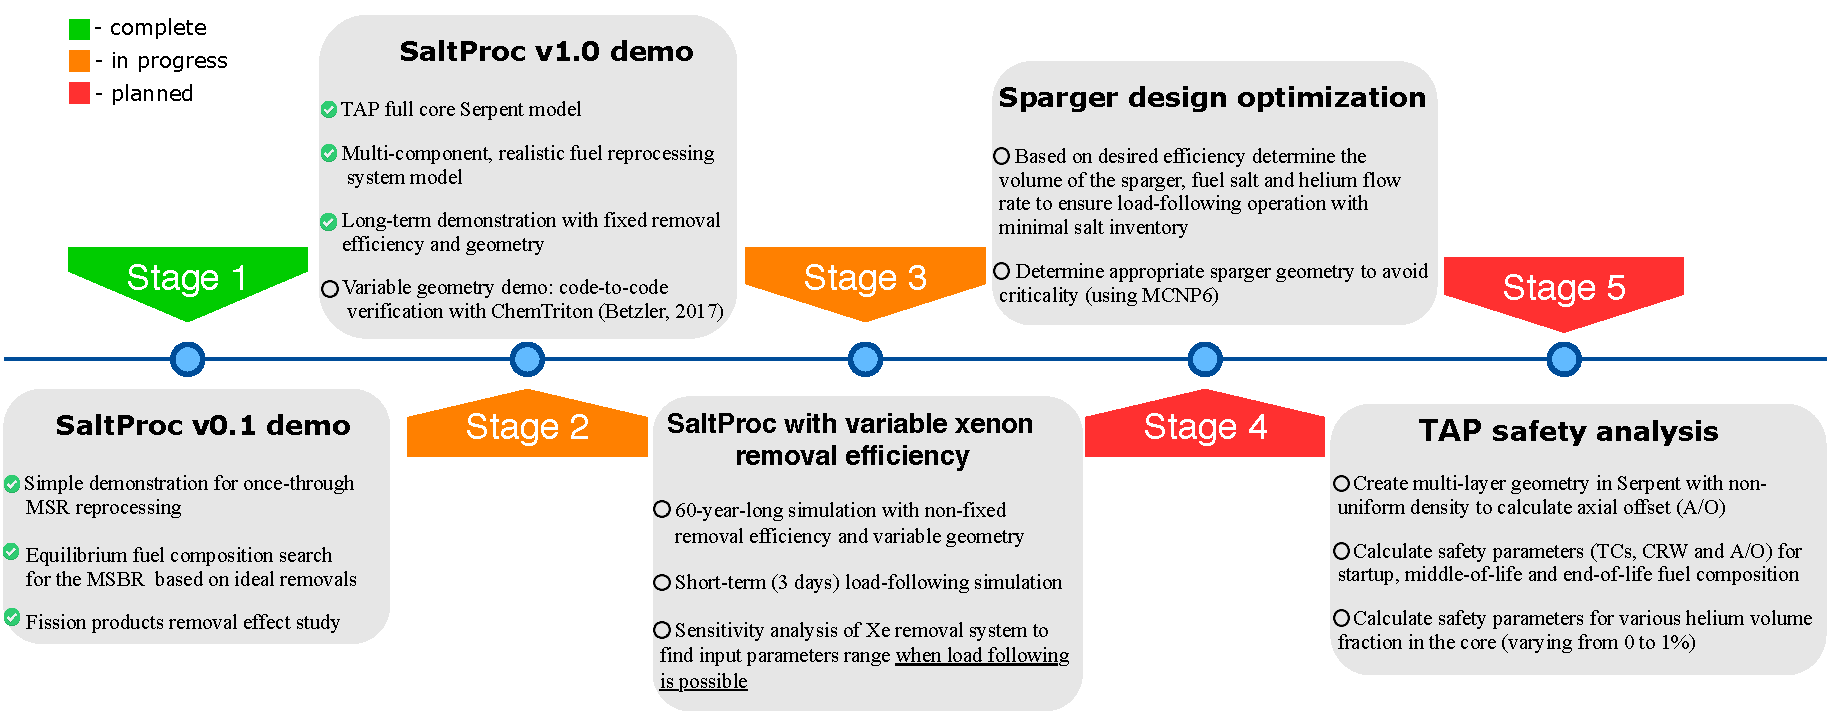
\includegraphics[width=1.06\textwidth]{progress_chart.pdf} 
 	\caption{Workflow for the simulations proposed in this work..}
 	\label{fig:workflow}
 \end{sidewaysfigure}
 \FloatBarrier
 
 
\section{Stage 1: basic online reprocessing demonstration}
At this stage \gls{MSR} online reprocessing capabilities has been reviewed and 
summarized (Chapter 1). SaltProc v1 was demonstrated for simplified burnup 
calculation for the \gls{MSBR} as a part of my M.Sc. thesis 
\cite{rykhlevskii_advanced_2018} and published paper 
\cite{rykhlevskii_modeling_2019}. These efforts illuminated depletion of the 
fuel salt in the \gls{MSBR} for 60 years of operation with taking into account 
following processes:
\begin{enumerate}
	\item \glspl{FP} removal from the salt with fixed, ideal extraction 
	efficiency (the fuel reprocessing system removed 100\% of target poison).
	\item 100\% of $^{233}$Pa being removed and equal mass of $^{233}$U is fed 
	into the core (instantaneous $^{233}$Pa decay to $^{233}$U was assumed).
	\item Fresh fertile material ($^{232}$Th) feed to maintain the fuel salt 
	inventory constant.
\end{enumerate}
Additionally, the effect of removing fission product from the fuel salt has 
been investigating separately for different group of \glspl{FP} (e.g., noble 
gases, noble ans seminoble metals, rare earth elements). As expected, removing 
fission products provide with significant neutronic benefit and enables a 
longer core lifetime. Section~\ref{sec:pre-results-msbr} described key 
findings after completing Stage 1.

\section{Stage 2: SaltProc v2.0+ demonstration and validation for the TAP}
Simulating realistic multi-component fuel reprocessing system is important for 
calculating an accurate fuel salt composition. SaltProc v1 was completely 
refactored for modeling a complicated salt reprocessing system. To demonstrate 
SaltProc v2.0+ capabilities, we have created a full-core \gls{TAP} 
\gls{MSR} model in Serpent 2 \cite{chaube_tap_2019} which was described in a 
detail in Section~\ref{sec:tap_model}. Moreover, the multi-component fuel 
reprocessing system of the \gls{TAP} was developed on this stage 
(Section~\ref{sec:stage2-demo}). Section~\ref{sec:stage2-demo} also presented 
preliminary results of Stage 2. Stage 2 demonstration case has following 
advantages over Stage 1:
\begin{itemize}
	\item SaltProc v1 (Stage 1) approximated the fuel salt reprocessing system 
	as a single ``black'' box, which removes entire mass (100\% removal 
	efficiency) of processed elements at once. In contrast, SaltProc v2.0+ 
	treats the fuel reprocessing system as complex structure of components 
	each removing specific set of elements with specific extraction 
	efficiency. 
	\item SaltProc v2.0+ inherently checks mass conservation at each depletion 
	step and dynamically calculates feed stream to maintain the salt inventory 
	constant.
	\item SaltProc v2.0+ tracks waste stream from each component.
\end{itemize}

Foremost future effort on this Stage is to implement capability of switching 
between multiple Serpent geometries during simulation. For the \gls{TAP} 
concept the number of moderator rods in the core varies from 1332 at the 
startup to 6700 at the \gls{EOL}. The user will have an option to choose when 
SaltProc v2.0+ should switch to next geometry: (1) after specific depletion  
time (e.g., 18 months which is a common maintenance/refueling 
shutdown interval for \glspl{LWR}); (2) effective multiplication factor 
reaches specific value (e.g., $1.0<k_{eff} < 1.01$). Additionally, SaltProc 
v2.0+ will correct the total fuel salt inventory in a primary loop to 
compensate the core geometry change. That is, after each moderator rods  
reconfiguration, excess of the fuel salt will be virtually ``drained'' in 
a separate tank, and this tank inventory will be stored in the database. 
Overall, the adjustable geometry capability will allow to realistically 
simulate long-term (60 years) operation of the \gls{TAP} reactor to obtain 
accurate fuel salt composition at different moments during operation.

Obtained at Stage 2 results will be used for code-to-code verification with  
ChemTriton/Shift results for full-core \gls{TAP} core geometry from the most 
recent \gls{ORNL} technical report TM-2017/475 \cite{betzler_assessment_2017} 
for confidence building. Notably, the fuel salt composition evolution during 
the \gls{TAP} reactor operation and corresponding core geometry are 
determinative for all next stages.

This work is developed with a test-driven development paradigm. Specifically, 
before any new functionality is implemented, a suite of tests is written which 
as closely define its expected behavior as possible. The code is then written 
with the goal of passing the test suite. In this way, the tool developed in 
this work is expected to be comprehensively tested in parallel with its 
development. Thus, after code-to-code verification with ChemTriton/Shift 
multiple-component integration test will be added to the test harness to make 
sure that future changes in the code will not break previous functionality.

Test problems will help comprehensively define and confirm each unit of the 
demonstration functionality. These problems will include very basic, 
information-passing tests as well as more challenging multiple-component 
integration tests. Every unit of functionality within the toolkit will be 
tested as an integral part of development.

This milestone will result in a processing system model capable of simulating
various liquid-fueled \gls{MSR} with multi-component fuel reprocessing system 
but with constant separation efficiency, defined at runtime. Additionally, 
this stage model will demonstrate a key feature of the \gls{TAP} \gls{MSR} - 
adjusting the moderator rods configuration - which is necessarily to maintain 
the reactor critical during 60 years lifetime. 

\section{Stage 3: variable xenon extraction rate}
When the Stage 2 is established, a series of extensions to these models will 
be pursued. These will incorporate extraction efficiencies as a function of 
many physical system design parameters (e.g., void fraction in the salt, 
helium bubble size). Mathematical correlations for the efficiencies will be 
taken from the literature \cite{peebles_removal_1968, 
gabbard_development_1974} and from CFD-simulations currently being conducted 
at the University of Illinois at Urbana-Champaign \cite{huff_enabling_2018}. 
For demonstration proposes, removal efficiency for xenon only will be defined 
as a function of liquid phase mass transfer coefficient, gas-liquid 
interfacial area and temperature (Section~\ref{sec:gas-separ}) because of 
limited experimental data provided in the listed literature. For other 
elements from the \gls{TAP} reprocessing scheme 
(table~\ref{tab:reprocessing_list}), removal efficiencies will be defined 
based on the removal rates from the table, assuming time-independent 
extraction efficiency. This milestone will result in a realistic online 
reprocessing system model capable of modeling \gls{MSR} systems with 
parameterized, realistically achievable process rates and extraction  
efficiencies.

To test the ability for \gls{TAP} reactor to operate in a load-following 
regime, short-term (1 week) depletion with the core power changing in range 
0-100\% with ramp rate 10\%/min will be simulated with SaltProc v2.0+. The 
depletion step time for this simulation will be varied in a range from 1 to 60 
min to compromise between accuracy of the result and cost. It is expected that 
load-following performance will be better in the \gls{BOL} because neutron 
energy spectrum thermalizes during the reactor operation. Thus, short-term 
load-following simulation will be repeated for the \gls{BOL}, 1 year after the 
startup, middle of life, and the \gls{EOL}.

Additionally, sensitivity analysis of input parameters in the xenon extraction 
correlation will be conducted to determine parameters(e.g., mass transfer 
coefficient) range when load-following is actually possible for the \gls{TAP} 
reactor in a worst-case scenario of power demand. These multiple inputs 
incorporating user-parametrized components in the fuel salt processing 
system will be collected and published in a \textit{.json}-compatible database 
for use with the SaltProc v2.0+ to encourage further research in this area.


\section{stuff}
For realistic removal rates and efficiencies, some fraction of neutron poisons 
will remain in the fuel salt and deteriorate the neutron economy. Even with 
fresh salt feed compensation of poison removal, the neutron multiplication 
factor will slowly decrease and eventually the \gls{MSR} core will become 
subcritical. The time before 
shutdown strongly depends on reprocessing facility performance 
and will be evaluated for realistic \gls{TAP} processing plant model 
in this work. Depending on time before shutdown, additional 
extension will 
incorporate a reactivity control module which injects more fissile 
material into the core when the reactor is close to subcritical state. 
In this case, the fraction of irradiated fuel salt from the outlet of 
the reactor vessel will be removed to conserve mass balance in the 
primary loop.

As the toolkit becomes capable of representing various reprocessing 
concepts, these will be analyzed for different full-core 
high-fidelity \gls{MSR} models discussed in Chapter 4. As discussed, 
these concepts will represent different processing challenges 
for various salt compositions, neutron spectra, and designs. 
Notably, the \gls{MSBR} reprocessing plant design is more complex 
than \gls{TAP}'s because it contains an additional protactinium 
isolation system with protactinium decay tank. Thus, a SaltProc 
demonstration for the \gls{MSBR} concept will test material decay 
in the protactinium decay tank using built-in PyNE capabilities. 
These models input data will be collected and 
published in a \textit{.json}-compatible database for use with the 
Python package to encourage further research in this area.



\subsection{Demonstration Case Development}
The proposed tool class structure and flowchart are 
described in detail in section~\ref{sec:tool_design}.
A first milestone in the development of this toolkit will be a 
principle demonstration of coupling with SERPENT 2 and 
information passing schemes. That is, no removals or feeds 
will be implemented in this demonstration stage. However, 
the component models will be developed in such way that 
they are capable of passing data about materials (e.g., isotopic 
composition vector) via set of \textit{Processes} but this 
processing system will not actually modify \textit{MaterialFlow} 
(separation efficiency is to be set 0\%).

The demonstration will produce a complete but `empty' processing 
model. It will simulate \gls{MSR} system operation during 
a long time period and obtain resulting fuel salt isotopic composition. 
After that, the result will be verified against fuel salt 
composition obtained with pure SEPRENT 2 output for the same 
depletion parameters and the core geometry.% because this case does not 
%introduce any online processing challenges.

At the subcomponent level, the demonstration will include information 
passing, bookkeeping, and mass balance within and between the 
subcomponents. Information passing between subcomponents 
(\textit{Processes}) concerning nuclide concentration, mass flow rate 
and total volume in \textit{MaterialFlow} will be implemented and tested. 
An HDF5 output database will contain 
isotopic composition vectors, simulation 
parameters, and all relevant processing information.

This work is developed with a test-driven development paradigm. 
Specifically, before any new functionality is implemented, a suite of 
tests is written which as closely define its expected behavior as 
possible. The code is then written with the goal of passing the test 
suite. In this way, the tool developed in this work is expected to be
comprehensively tested in parallel with its development.

Test problems will help comprehensively define and confirm each unit 
of the demonstration functionality. These problems will include very 
basic, information-passing tests as well as more challenging multiple-
component integration tests. Every unit of functionality
within the toolkit will be tested as an integral part of development.

When the unit test suite passes, validation efforts against results 
in the literature will demonstrate that the complete 
processing system model behaves in agreement with previous research 
efforts \cite{rykhlevskii_advanced_2018, rykhlevskii_modeling_2019}. 
If it does not behave as expected, sensitivity analyses, 
model abstraction, and computational development will be iteratively 
conducted until the model is validated.

\subsection{Base Case Development}
The next stage in this work will be the development of the base case. 
This will build upon the demonstration processing system model by 
implementing simplified physics for each of the subcomponents. This 
will include constant non-ideal extraction efficiency which is 
different for each target chemical element. Moreover, a realistic 
model of the conceptual \gls{TAP} reprocessing plant involving 
multiple processes (serial and parallel) will be implemented on this 
stage. 

Additional information such as void fraction, helium 
bubble size and other component-specific, user-defined 
parameters will be added to the demonstration case model.
Also this will include non-zero fuel salt feed which 
compensate the removed poisons mass loss in a primary loop.
This milestone will result in a processing system model capable of 
modeling various liquid-fueled \gls{MSR} with comprehensive 
online reprocessing system but with constant separation efficiency, 
defined at runtime.

Unit testing, verification and validation will occur in a manner 
very similar to the previous case. Unit tests will assess the 
performance of each extension functionality as well as their 
integrated behavior. Validation against existing results for 
\gls{TAP} obtained by ChemTriton \cite{betzler_two-dimensional_2017, 
betzler_molten_2017} will also be performed for confidence 
building. The high-fidelity full-core \gls{TAP} model for 
SERPENT 2 has been developed already and described in detail 
in section~\ref{sec:tap_model}.

Additionally, the base case model will be used to estimate effective 
multiplication factor ($k_{eff}$) dynamics for long-time 
depletion simulations. Particularly, $k_{eff}$ change overtime 
will demonstrate 
ability of the \gls{TAP} system to maintain a critical state with a
fresh salt feed rate equal separated neutron poison loss rate. 
To avoid subcriticality, an additional reactivity 
controlling subcomponent will be implemented on the extension stage. 
This subcomponent 
will inject additional fissile material 
when $k_{eff}$ for the core drops below a specific value (e.g., 
$k_{eff}<1.01$) and will then repeat the previous depletion step. 
This module will enable maintenance of reactor criticality 
throughout reactor operation.
 
\subsection{Extension Development}
When the base case is established, a series of extensions to 
these models will be pursued. These will incorporate extraction 
efficiencies as a function of many physical system design 
parameters. Mathematical correlations for the efficiencies will 
be taken from the literature \cite{gabbard_development_1974}, 
experiments and from CFD-simulations currently being conducted at 
the University of Illinois at Urbana-Champaign \cite{huff_enabling_2018}.
This milestone will result in a realistic online reprocessing system 
model capable of modeling \gls{MSR} systems with realistically achievable 
process rates and efficiencies as well as variable feed streams. 

For realistic removal rates and efficiencies, some fraction of neutron 
poisons will remain in the fuel salt and deteriorate the neutron 
economy. Even with fresh salt feed compensation of poison removal, 
the neutron multiplication factor will slowly decrease and 
eventually the \gls{MSR} core will become subcritical. The time before 
shutdown strongly depends on reprocessing facility performance 
and will be evaluated for realistic \gls{TAP} processing plant model 
in this work. Depending on time before shutdown, additional 
extension will 
incorporate a reactivity control module which injects more fissile 
material into the core when the reactor is close to subcritical state. 
In this case, the fraction of irradiated fuel salt from the outlet of 
the reactor vessel will be removed to conserve mass balance in the 
primary loop.

As the toolkit becomes capable of representing various reprocessing 
concepts, these will be analyzed for different full-core 
high-fidelity \gls{MSR} models discussed in Chapter 4. As discussed, 
these concepts will represent different processing challenges 
for various salt compositions, neutron spectra, and designs. 
Notably, the \gls{MSBR} reprocessing plant design is more complex 
than \gls{TAP}'s because it contains an additional protactinium 
isolation system with protactinium decay tank. Thus, a SaltProc 
demonstration for the \gls{MSBR} concept will test material decay 
in the protactinium decay tank using built-in PyNE capabilities. 
These models input data will be collected and 
published in a \textit{.json}-compatible database for use with the 
Python package to encourage further research in this area.

\subsection{Sensitivity Analysis}
Experimental data for removal efficiencies is very limited and lack 
fidelity of the correlations. Salt flow rate, system volume, 
void fraction, helium bubble size (for volatile gases removal), 
temperature, pressure, and material properties are uncertain due to 
limited experimental data. These information will impact the 
processing system extraction efficiencies. As a part of this work, 
uncertain or flexible model input parameters will be sampled randomly 
from an appropriate distribution to obtain corresponding output 
distributions. These resulting distributions can be used to estimate 
system components design and safety margins. Furthermore, it will 
provide helpful insights to identify impactful parameters and 
find key performance drivers for reprocessing system design.

While it is out of the scope of this work to perform comprehensive 
analysis and optimization of various \glspl{MSR} systems, this 
work seeks to provide a tool which would be helpful to perform such 
analyses. Thus, some limited analysis of \gls{MSR} fuel cycle 
performance including estimation of breeding ratio, fuel utilization, 
mass of waste disposed and recovered will be performed to demonstrate 
that the tools developed in this work can illustrate the sensitivity 
of processing plant performance to conceptual nuclear system parameters.


The final extension stage will build be upon the base case by 
implementing extending physics and chemistry correlations for 
extraction efficiencies to capture impact of non-ideal 
removal rates on the reactor performance modeling. These 
stages will be completed during a test-driven software 
development approach, will leverage unit tests and 
continuous integration for sustainable development. Finally, 
data collected during these stages will be organized and 
published in a \textit{.json} format data library for use 
with the SaltProc Python package.

Additionally, sensitivity analysis for the \gls{TAP} fuel processing 
system design will be performed to determine desirable ranges 
for principal system parameters. Particularly, inputs to the 
system model (e.g., components volumes, holdup capacities, helium 
bubble size, etc) will be sampled from appropriate 
distributions to obtain results (e.g., fuel utilization) in the 
form of corresponding distributions. These data later will be used
to formulate design requirements and safety margins for 
\gls{MSR}'s reprocessing system.